\documentclass[10pt,a4paper]{article}
\usepackage[margin=2.2cm]{geometry}
\usepackage{fontspec}
\usepackage{kotex}
\setmainfont{Apple SD Gothic Neo}
\setsansfont{Apple SD Gothic Neo}
\usepackage{amsmath,amssymb}
\usepackage{graphicx}
\usepackage{booktabs}
\usepackage{caption}
\usepackage[dvipsnames]{xcolor}
\usepackage[colorlinks=true,linkcolor=MidnightBlue,citecolor=MidnightBlue,
            urlcolor=MidnightBlue]{hyperref}
\usepackage{titlesec}
\titleformat{\section}{\large\bfseries}{\thesection}{0.6em}{}
\captionsetup{font=small,labelfont=bf}
\setlength{\parskip}{0.35em}
\setlength{\parindent}{0pt}

\usepackage{mdframed}
\newmdenv[linewidth=0.4pt,linecolor=gray!60,backgroundcolor=gray!5,
          innertopmargin=6pt,innerbottommargin=6pt,skipabove=8pt,skipbelow=8pt]{claimbox}
\newcommand{\claim}[2]{\begin{claimbox}\textbf{주장.} #1\par\smallskip
  \textcolor{gray!70}{\textbf{반증 조건.} #2}\end{claimbox}}

\title{\bfseries 폐기 확정의 발밑\\[2pt]
\large 앱은 서고 KR 은 물러난다 --- 그리고 합성 자 $3$부작의 종결}
\author{월드모델 실험실 · 노트 $832{\sim}833$}
\date{2026-08-07}
\begin{document}\maketitle

\section{한 줄 둘}

\textbf{①($833$)} $821/822$ 의 ``두 짝 모두 릿지 승 --- 온보딩 서사 폐기
확정''은 상수 자($2$배 오기판) 위 판정이었다. 규약 $47$ 자(군집 BCa · 앙상블
전이)로 재채점: \textbf{비게임 앱 $\Delta +0.2006$ $[+0.093, +0.323]$ 릿지승
유지} · \textbf{KR 만화 $\Delta +0.0423$ $[-0.030, +0.120]$ 판정 불능}(예측
$60\%$ 적중 --- $1$차 원리로 반폭 $\pm 0.09{\sim}0.11$ 을 미리 적었다). 사업
문장 수정: \emph{``앱에서 확정 · KR 은 방향 일치·크기 미확정''} --- 판권
숫자에서 KR 격차는 뺀다. \textbf{폐기 자체는 앱 하나로 선다} --- 전이 우위가
성립하는 짝은 $0$ 이다.

\textbf{②($832$a/b)} 곡선 자 갈래 종결 --- 결합 자는 같은형태 위양성
$8.3\% > 5\%$ 로 기각(원천: 특징 자의 다봉 분산 과민), 안정화(재생성 평균)는
p$95$ 를 비례 축소시켜 위양성률 불변. 최종 능력 카드: \textbf{곡선 형태
판별에서 팔 수 있는 것은 `RMSE $>3\times$쌍바닥 $+$ 합동 널 초과'의
`다르다'뿐.} 다음 문은 KOBIS 실측 곡선이다.

\begin{figure}[t]\centering
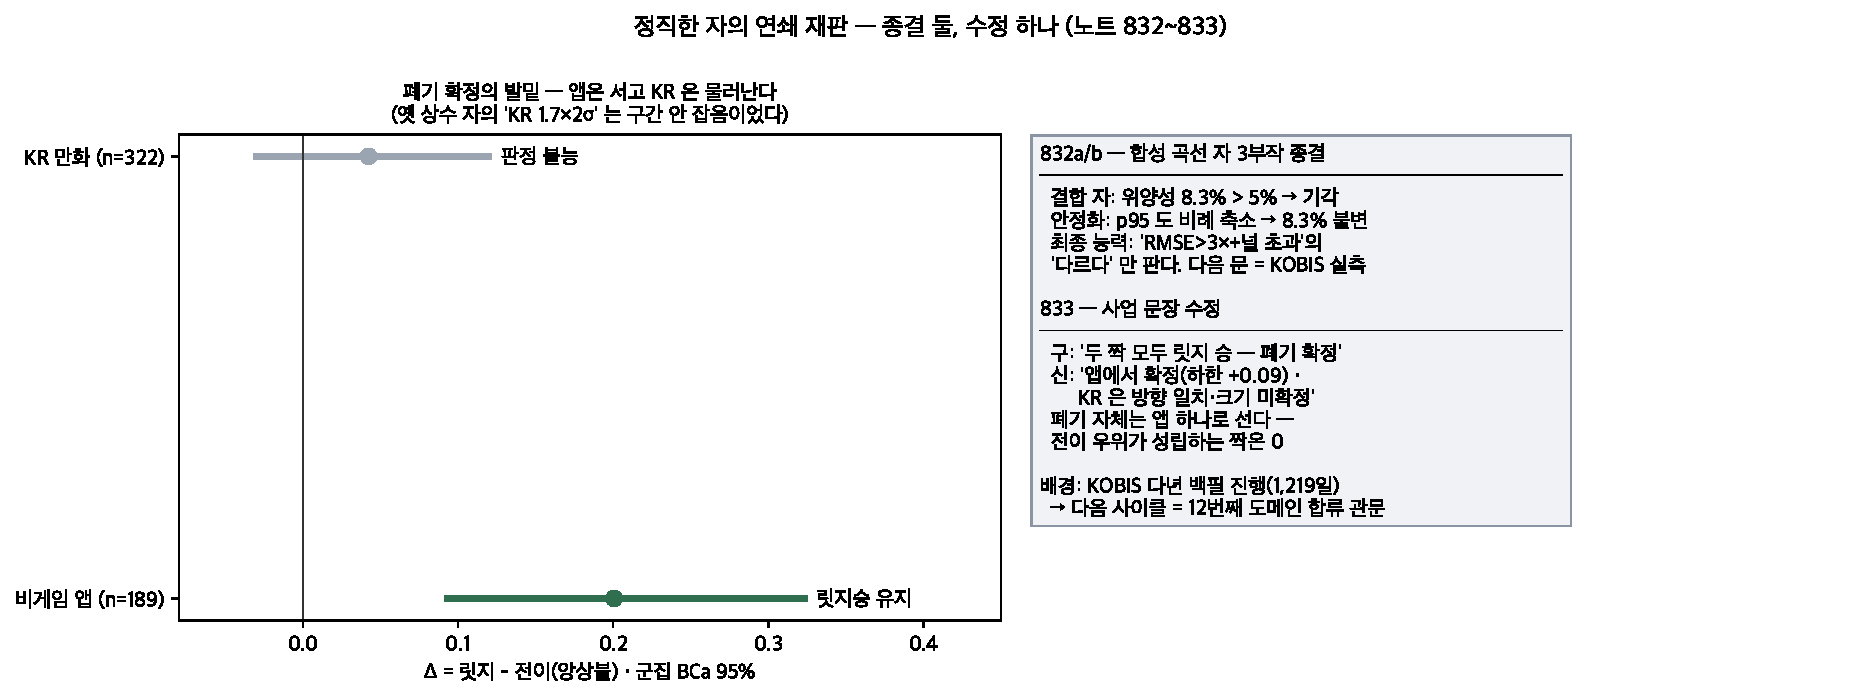
\includegraphics[width=0.97\textwidth]{figs/foot.pdf}
\caption{왼쪽: 두 짝의 $\Delta$ 구간. 오른쪽: 사이클 요약.}
\end{figure}

\section{남는 것}

\claim{\textbf{정직한 자의 연쇄 재판이 닫혔다} --- $827$(지도) · $828$(정오표)
· $832$(곡선 자) · $833$(짝 격차)로 상수 자 시대의 판정 전부가 재채점됐다.
살아남은 것: 합동승 $5$ · 앱 릿지승 · $825$ 통과. 물러난 것: 아이돌 릿지승 ·
시장팝업 챌린저 승 · KR 릿지승 · 곡선 형태 자 일체. \textbf{남은 판정 부채는
$0$ 이다.}}
{배경에서 KOBIS 다년 백필($1{,}219$일)이 돌고 있다 --- 다음 사이클이 $12$번째
도메인 합류 관문(q$85$ 재산출 · K$=21$ 라벨 성립률 · 취소 조건 · 재기선 절차)을
집행한다. 판 $\rho$ $0.4689$ 그대로 --- 합류가 성사되면 재기선이다.}

\end{document}
